\documentclass[a4paper,11pt]{article}

\usepackage[T1]{fontenc}
\usepackage[utf8]{inputenc}
\usepackage{graphicx}
\usepackage{xcolor}

\renewcommand\familydefault{\sfdefault}
\usepackage{tgheros}
\usepackage[defaultmono]{droidmono}

\usepackage{amsmath,amssymb,amsthm,textcomp}
\usepackage{enumerate}
\usepackage{multicol}
\usepackage{tikz}

\usepackage{geometry}
\geometry{left=25mm,right=25mm,%
bindingoffset=0mm, top=20mm,bottom=20mm}


\linespread{1.3}

\newcommand{\linia}{\rule{\linewidth}{0.5pt}}

% custom theorems if needed
\newtheoremstyle{mytheor}
    {1ex}{1ex}{\normalfont}{0pt}{\scshape}{.}{1ex}
    {{\thmname{#1 }}{\thmnumber{#2}}{\thmnote{ (#3)}}}

\theoremstyle{mytheor}
\newtheorem{defi}{Definition}

% my own titles
\makeatletter
\renewcommand{\maketitle}{
\begin{center}
\vspace{2ex}
{\huge \textsc{\@title}}
\vspace{1ex}
\\
\linia\\
\@author \hfill \@date
\vspace{4ex}
\end{center}
}
\makeatother
%%%

% custom footers and headers
\usepackage{fancyhdr}
\pagestyle{fancy}
\lhead{}
\chead{}
\rhead{}
\lfoot{UFO - Assignment 2}
\cfoot{}
\rfoot{Page \thepage}
\renewcommand{\headrulewidth}{0pt}
\renewcommand{\footrulewidth}{0pt}
%

% code listing settings
\usepackage{listings}
\lstset{
    language=Java,
    basicstyle=\ttfamily\small,
    aboveskip={1.0\baselineskip},
    belowskip={1.0\baselineskip},
    columns=fixed,
    extendedchars=true,
    breaklines=true,
    tabsize=4,
    prebreak=\raisebox{0ex}[0ex][0ex]{\ensuremath{\hookleftarrow}},
    frame=lines,
    showtabs=false,
    showspaces=false,
    showstringspaces=false,
    keywordstyle=\color[rgb]{0.627,0.126,0.941},
    commentstyle=\color[rgb]{0.133,0.545,0.133},
    stringstyle=\color[rgb]{01,0,0},
    numbers=left,
    numberstyle=\small,
    stepnumber=1,
    numbersep=10pt,
    captionpos=t,
    escapeinside={\%*}{*)}
}

\usepackage{graphicx}
\graphicspath{ {./assets/} }

\usepackage{hyperref}
\hypersetup{
    colorlinks=true,
    linkcolor=blue,
    filecolor=magenta,      
    urlcolor=cyan,
}

%%%----------%%%----------%%%----------%%%----------%%%

\begin{document}

\title{UFO - Assignment 2}

\author{Adam Lass, Rasmus Helsgaun, Stephan Djurhuus, Pernille Lørup}

\date{24/11/2020}

\maketitle

\section*{Objectives}

You need to make it run at least 50\% faster than it is now, and should be able to get to around 100\% faster. 
\\*Hand-in: should contain the following:

\begin{itemize}
  \item Documentation of the current performance (remember mean and standard deviation -- see the Sestoft paper!)
  \item An explanation of the bottlenecks in the program.
  \item A hypothesis of what is causing the problem,
  \item A changed program which is improved to solve the problem.
  \item Documentation of the new performance.
\end{itemize}

\emph{Notice: there might be more than one optimization needed to achieve optimal performance.}

\section*{Hypothesis \& Bottlenecks}

A call is made to read a system file each time \textbf{FileReader} is called. A \textbf{FileReader} will make 256 calls for reading 256 characters from file.\\*
\textbf{try/catch} is reducing the performance due to its check and preparation of potential exceptions.

\begin{lstlisting}[label={list:first}]
private static void tallyChars(Reader reader, Map<Integer, Long> freq) throws IOException {
    int b;
    while ((b = reader.read()) != -1) {
        try {
            freq.put(b, freq.get(b) + 1);
        } catch (NullPointerException np) {
            freq.put(b, 1L);
        };
    }
}
\end{lstlisting}

\section*{Optimization}

\subsection*{Tally Chars Custom 1}

This method uses \textbf{freq.getOrDefault} instead of using \textbf{try/catch} that checks if the \textbf{Key} exists and then throws an exception if it doesn't.

\begin{lstlisting}[label={list:second}]
private static void tallyCharsCustom1(Reader reader, Map<Integer, Long> freq) throws IOException {
    int b;
    while ((b = reader.read()) != -1) {
        freq.put(b, freq.getOrDefault(b, 0L) + 1L);
    }
}
\end{lstlisting}

\subsection*{Tally Chars Custom 2}

In addition to \textbf{tallyCharsCustom1} this method makes use of the \textbf{BufferedReader} which uses a memory buffer to optimize reading time.

\begin{lstlisting}[label={list:third}]
private static void tallyCharsCustom2(Reader reader, Map<Integer, Long> freq) throws IOException {
    int b;
    BufferedReader br = new BufferedReader(reader);

    while ((b = br.read()) != -1) {
        freq.put(b, freq.getOrDefault(b, 0L) + 1L);
    }
}
\end{lstlisting}

\newpage 
\subsection*{Tally Chars Custom 3}

Using \textbf{byte[]} optimizes performance because it is a simple data structure. This reduces unnecessary operations and therefore optimizes performance time.

\begin{lstlisting}[label={list:third}]
private static void tallyCharsCustom3(byte [] fileBytes, Map<Integer, Long> freq) throws IOException {
    int singleInt;
    for(byte b : fileBytes) {
        singleInt = (int) b;
        freq.put(singleInt, freq.getOrDefault(singleInt, 0L) + 1);
    }
}
\end{lstlisting}

\section*{Performance}

\subsection*{Tally Chars}
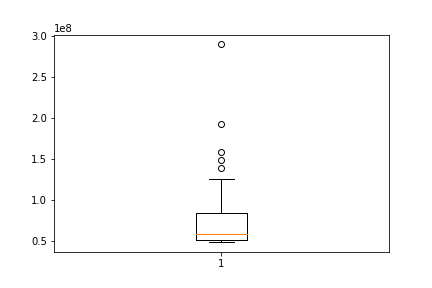
\includegraphics{assets/Tally_Chars.png} 

\noindent std: 44704672.3019 \\
mean: 77245155.5800

\subsection*{Tally Chars Custom 1}
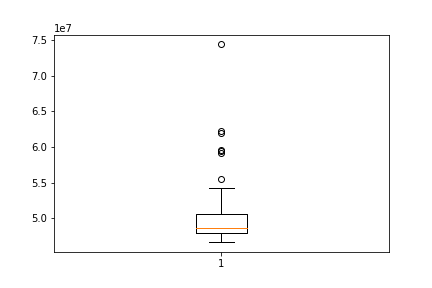
\includegraphics{assets/Tally_Chars_Custom_1.png}

\noindent std: 5212312.7555 \\
mean: 50741955.4000

\subsection*{Tally Chars Custom 2}
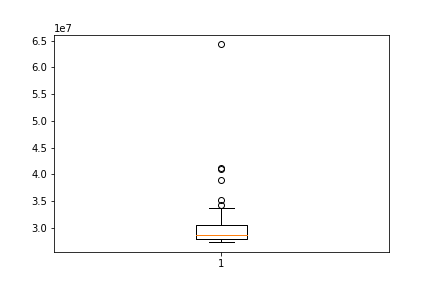
\includegraphics{assets/Tally_Chars_Custom_2.png}

\noindent std: 5884498.2695 \\
mean: 30583595.9400

\subsection*{Tally Chars Custom 3}
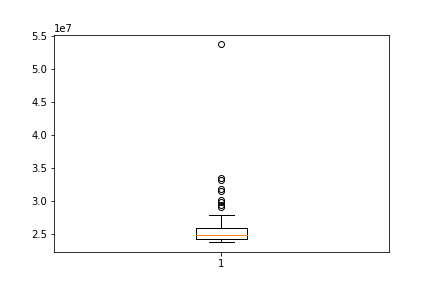
\includegraphics{assets/Tally_Chars_Custom_3.png}

\noindent std: 4698149.1470 \\
mean: 26328980.2800

\subsection*{Specifications}
The code was executed on a MacBook Pro (Retina, 13-inch, Early 2015) with a 2,9 GHz Dual-Core Intel Core i5 Processor. The MacBook has a memory of 8 GB 1867 MHz DDR3.\\*
The code was executed with Java version 13.0.2.

\subsection*{Conclusion}

The third alteration of the the \textbf{tallyChars} method has the best performance with approximately \textbf{293.38\%}

\section*{Resources}
We used a \href{https://github.com/Soft20/UFO-Assignment-2/blob/main/src/analysis/notebook.ipynb}{Jupyter Notebook} to analyse the \href{https://github.com/Soft20/UFO-Assignment-2/blob/main/src/analysis/observations.csv}{collected performance data}.

\noindent \href{https://github.com/Soft20/UFO-Assignment-2/blob/main/src/main/java/cphbusiness/ufo/letterfrequencies/Main.java}{Java code solution}

\end{document}
